\documentclass[conference]{style/IEEEtran}
\IEEEoverridecommandlockouts
\usepackage{cite}
\usepackage{amsmath,amssymb,amsfonts}
\usepackage{algorithmic}
\usepackage{graphicx}
\usepackage{textcomp}
\usepackage{xcolor}
\def\BibTeX{{\rm B\kern-.05em{\sc i\kern-.025em b}\kern-.08em
    T\kern-.1667em\lower.7ex\hbox{E}\kern-.125emX}}

%\usepackage{biblatex}
%\addbibresource{references/references.bib}
    
\begin{document}
\title{A methodological framework to enable the roaming agreement digitization: An NLP-based approach\\}

\maketitle

\begin{abstract}
This document is a model and instructions for \LaTeX.
This and the IEEEtran.cls file define the components of your paper [title, text, heads, etc.]. *CRITICAL: Do Not Use Symbols, Special Characters, Footnotes, 
or Math in Paper Title or Abstract.
\end{abstract}

\begin{IEEEkeywords}
component, formatting, style, styling, insert
\end{IEEEkeywords}

\section{Introduction}
The roaming service maintains the persistent connectivity of subscribers in different networks and locations. Roaming describes the capability of a subscriber to access mobile services offered by the visited public mobile network (VPMN) through the home public mobile network (HPMN), when roaming outside the coverage range of the HPMN \cite{b1}. However, before ensuring persistent connectivity the Mobile Network Operators (MNOs) must reach an agreement regarding the technical, commercial and legal relationships known as the Roaming Agreement (RA).

In order to standardize technical, commercial and legal aspects of RA, the GSM Association broadly outlines the content of such RA in standardized form for its members \cite{b2}. Reference \cite{b3} provides a list of the most commonly used GSMA standards, which are summarized bellow: (1) AA.12 constitutes a standard GSMA or Permanent Reference Document; (2) AA.13 contains the common annexes with operational information (e.g., information on tap file, billing data, settlement procedure, customer care, fraud, etc.) and (3) AA.14 involves the individual annexes containing information about the operator (e.g., contact details of the roaming team, fraud team, IREG team, TADIG team, etc.).

While it is true that it is not mandatory to follow the standards proposed by GSMA, according to authoritative voices in the field of negotiating RA drafting, most MNOs follow them strictly \cite{b4}. Therefore, a first point to consider in the RA drafting is how far it is deviated from the GSMA's proposed standards. Thus, during the drafting process of the agreement, the parties should analyze the sub-articles contained in the GSMA standard templates to determine whether:

\begin{enumerate}
\item Specify the value of certain \textit{variables} that are found in a certain text, such as dates, names of entities, amounts and others.

\item Leave an article/sub-article as found in the template thereby establishing a \textit{standard clause}.

\item Introduce certain \textit{variations} in the articles/sub-articles, by changing \textit{variables}, e.g., MNO, dates, penalties, currencies and so on with respect to the original text, i.e., the GSMA templates.

\item Introduce completely new articles/sub-articles that respond to particular interests by constituting \textit{customized texts}.

\end{enumerate}

However, a successful RA drafting goes through a complex negotiation process in which, currently the parties, i.e. the Mobile Network Operators (MNOs), still use asynchronous flows such as email or even regular mail for information exchange. Since these processes lack transparency, which can result in the violation of the RA by MNOs, it is necessary to provide a transparent digitization system for RA drafting negotiations. For this reason, this paper proposes the use of Natural Language Processing (NLP) as an engine to digitize the legal text as a starting point of a RA transparent drafting process. The NLP engine analyzes the different articles and sub-articles of the RA determining the existence of variables, variations, standard clauses and customized texts in the text. For this purpose, on the one hand, NLP techniques such as Named Entity Recognition (NER) and Part of Speech (POS) are applied from an unstructured data information discovery tools such as \textit{Amazon Comprehend} and on the other hand, a comprehensive comparison between texts is established based on \textit{similarity} determination techniques. Both techniques are integrated as part of the development of an unstructured text processing tool that integrates an specific methodology for the use case, i.e., a transparent digitization of roaming agreements.

The rest of this manuscript is structured as follows: Section 2 reviews both attempts at a transparent digitization of Roaming Agreement and existing NLP-based digitization mechanisms as part of the related work. Section 3 establishes the designed methodology. The implementation of our system are described in Section 4. Section 6 discusses the results of conducted experiments. Finally, the conclusions of the manuscript are included in Section 7.

\section{Related work}

Both in the scientific literature and in business environments there are important approaches to RA digitalization. Thus, the reference \cite{b5} proposes a dynamic RA between the Local 5G Operator and the MNO. The interaction between the two entities takes place through an Ethereum based platform. A second approach focuses uniquely on the billing of the services obtained as a result of the RA \cite{b6}. This agreement is incorporated as part of a smart contract so the work contributes significantly to the digitization process of the agreement, allowing for a faster, more seamless process in which payments can be requested and obtained quickly due to less need for manual intervention. The contextualization of this system in the business environment is proposed by important MNOs such as Telefonica, Deutsche Telekom and Vodafone which use blockchain for Roaming settlement within the framework of the RA between the parties \cite{b7}. However, these contributions are focused from a RA technical perspective rather than the context of a transparent digitization to enhance the negotiation process for the effective drafting of the roaming agreement. 

Additionally, the scientific literature addresses text processing systems based on nlp techniques in domains such as judiciary. Thus, the reference \cite{b9} addresses the process of digitization in the judicial sectors from archives of court records for which the authors have designed a textual analysis tool that includes grammatical analysis of documents in English based on NLP techniques. This linguistic analysis attempts to find the appropriate meaning of terms within a document. In addition, the reference \cite{b8} applies NLP-based processing techniques for information retrieval from spreadsheets and describes technologies for storing and retrieving database information. NLP techniques such as sentence tokenization, word tokenization, removing stopwords and lemmatization are part of the parsing stage of the work. Finally, authors of reference \cite{b10} propose a model for implementing sentimental analysis using Amazon Comprehend. This system performs an audio-to-text transcription and then performs the processing of the obtained text. Although these studies  constitute a relevant part of related work, e.g., by integrating useful tools such as Amazon Comprehend or detailing the use of techniques such as tokenization, the scientific literature does not address scenarios for the telecom field and even less in the context of a transparent digitization of the roaming agreement. Therefore, we can affirm that our work introduces a topic with a high degree of novelty.

\section{NLP Engine methodology}
Overall, the logic designed for the NLP engine follows two approaches: detection and comparison. Detection represents the capability to locate \textit{variables} in a text file, i.e., the Roaming Agreement. Comparison represents the capacity to find \textit{similarities} and differences between the sub-articles present in the Roaming Agreement with respect to the sub-articles present in the GSMA standard template. For example, while an almost total coincidence between texts at the sub-article level represents a \textit{standard clause}, an almost null coincidence between texts (or simply the non-existence of a sub-article of the GSMA standard template in the Roaming Agreement) represents a \textit{customized text}. Thus, the intermediate case is represented by the \textit{variation} in which there is a high coincidence between sub-articles and the existing differences are given by the presence of \textit{variables} such as the name of the MNO and the start date of the agreement. The technologies that enable both detection and comparison are discussed below as part of the \textit{background}. The third section integrates these tools as part of the designed methodology.

\subsection{Amazon comprehend}
In short, \textit{Amazon Comprehend} is a service that uses NLP techniques to extract insights about the content document by recognizing  the  entities,  key  phrases,  language,  sentiments,  and  other  common  elements  in  a  text \cite{b11}. The capabilities that \textit{Amazon Comprehend} integrates are key to the \textit{detection} approach.

\subsection{Similarity Analysis}
Similarity is used to compare different types of data, so it is a resource used for pattern classification, clustering and information retrieval problems \cite{b12}. Therefore, the similarity falls within the comparison approach. In this regard, our work distinguishes between two types of similarities: Jaccard similarity and Cosine similarity \cite{b13}. While the first one is established as the size of the intersection divided by the size of the union of two sets, the second one implies the determination of the cosine of the angle between two vectors.

\subsection{Designed Methodology}
Define abbreviations and acronyms the first time they are used in the text.

\section{Implemented System}
The Fig.~\ref{fig1} shows a overall architecture of the NLP Engine that integrates over a docker infrastructure, establishing as inputs the Roaming Agreement text file, as well as the GSMA standard templates; as processing layer the logic associated to the NLP Engine and as output the classification of sub-articles as \textit{standard clauses}, \textit{customized texts} and \textit{variations} depending of the \textit{variables} detection.

\begin{figure}[htbp]
\centerline{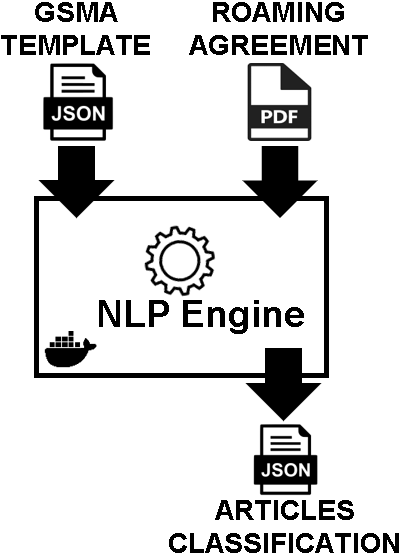
\includegraphics[width=0.25\textwidth]{images/NLP_Engine.png}}
\caption{NLP Engine overall architecture.}
\label{fig1}
\end{figure}

The first consideration regarding the developed architecture is that the NLP engine has been developed as a Software Development Kit and therefore it must be downloaded and executed from an entry point. 

\section{Discussion of Results}
Define abbreviations and acronyms the first time they are used in the text

\section{Conclusions}
Define abbreviations and acronyms the first time they are used in the text 


%\printbibliography

%\cite{erwerda2018}

\begin{thebibliography}{00}

\bibitem{b1} I. Tanaka, "Volte roaming and interconnection standard technology", NTT Docomo Technical Journal, vol. 15, no. 2, pp. 37-41, 2013.

\bibitem{b2} Ferwerda, R.; Bayings, M.; Van der Kam, M.; Bekkers, R. Advancing E-Roaming in Europe: Towards a Single “Language” for the European Charging Infrastructure. World Electr. Veh. J. 2018, 9, 50. https://doi.org/10.3390/wevj9040050.

\bibitem{b3} ROCCO, “The International Roaming Agreement,” 2017. [Online]. Available: https://www.roccoresearch.com/portfolio-items/the-roaming-agreement/. [Accessed: 24-Ago-2021].

\bibitem{b4} ROCCO, “What is ROAMING HUBBING?,” 2017. [Online]. Available: https://www.roccoresearch.com/portfolio-items/roaming-hubbing/. [Accessed: 24-Ago-2021].

\bibitem{b5} N. Weerasinghe, T. Hewa, M. Dissanayake, M. Ylianttila and M. Liyanage, "Blockchain-based Roaming and Offload Service Platform for Local 5G Operators," 2021 IEEE 18th Annual Consumer Communications and Networking Conference (CCNC), 2021, pp. 1-6, doi: 10.1109/CCNC49032.2021.9369516.

\bibitem{b6} C. Harris, "Improving Telecom Industry Processes Using Ordered Transactions in Hyperledger Fabric," 2019 IEEE Globecom Workshops (GC Wkshps), 2019, pp. 1-6, doi: 10.1109/GCWkshps45667.2019.9024541.

\bibitem{b7} M. Huillet, "Telefónica, Deutsche Telekom and Vodafone Use Blockchain for Roaming Settlement," 2020. [Online]. Available: https://cointelegraph.com/news/telefonica-deutsche-telekom-and-vodafone-use-blockchain-for-roaming-settlement. [Accessed: 24-Ago-2021].

\bibitem{b8} M. B.C., A. K., M. Y. M., R. L.R. and S. S.R., "Intelligent Automated Text Processing System - An NLP Based Approach," 2020 5th International Conference on Communication and Electronics Systems (ICCES), 2020, pp. 1026-1030, doi: 10.1109/ICCES48766.2020.9138070.

\bibitem{b9} M. A. Islam and M. Jahidul Haque, "Evaluating Document Analysis with kNN Based Approaches in Judicial Offices of Bangladesh," 2018 Second International Conference on Computing Methodologies and Communication (ICCMC), 2018, pp. 646-650, doi: 10.1109/ICCMC.2018.8487847.

\bibitem{b10} G. Satyanarayana, J. Bhuvana and M. Balamurugan, "Sentimental Analysis on voice using AWS Comprehend," 2020 International Conference on Computer Communication and Informatics (ICCCI), 2020, pp. 1-4, doi: 10.1109/ICCCI48352.2020.9104105.

\bibitem{b11} AWS, “Amazon Comprehend Developer Guide,” 2021. [Online]. Available: https://docs.aws.amazon.com/comprehend/latest/dg/comprehend-dg.pdf. [Accessed: 24-Jul-2021].

\bibitem{b12} J. Santisteban and J. Tejada-Cárcamo, "Unilateral Weighted Jaccard Coefficient for NLP," 2015 Fourteenth Mexican International Conference on Artificial Intelligence (MICAI), 2015, pp. 14-20, doi: 10.1109/MICAI.2015.9.

\bibitem{b13} S. Gupta, “Overview of Text Similarity Metrics in Python,” May 15, 2018, 2018. [Online]. Available: https://towardsdatascience.com/overview-of-text-similarity-metrics-3397c4601f50. [Accessed: 25-Jul-2021].

\end{thebibliography}

\vspace{12pt}

\end{document}
